
    Modern data centers are increasingly being provisioned with compute accelerators such as GPUs, FPGAs and ASIC's to catch up with the workload performance demands and reduce the total cost of ownership (TCO) \cite{caulfield2016cloud}. By 2021, traffic within hyperscale datacenters is expected to quadruple with 94\% of workloads moving to cloud-based datacenters according to Cisco's global cloud index~\cite{cisco}. Based on the nature of the application, it can either benefit from high throughput of GPUs or low latency of special purpose hardwares such as FPGAs and TPUs~\cite{jouppi2017datacenter}. A majority of them include data mining, image processing, speech recognition and gaming \cite{1659988, Povey11thekaldi,10.1007/11744023_32}, uses GPUs for high throughput computing. This trend is evident as public cloud operators like Amazon \cite{amazon} and Microsoft \cite{microsoft} have started to offer GPU-based infrastructure services.

\begin{figure}[!tbp]
\centering
  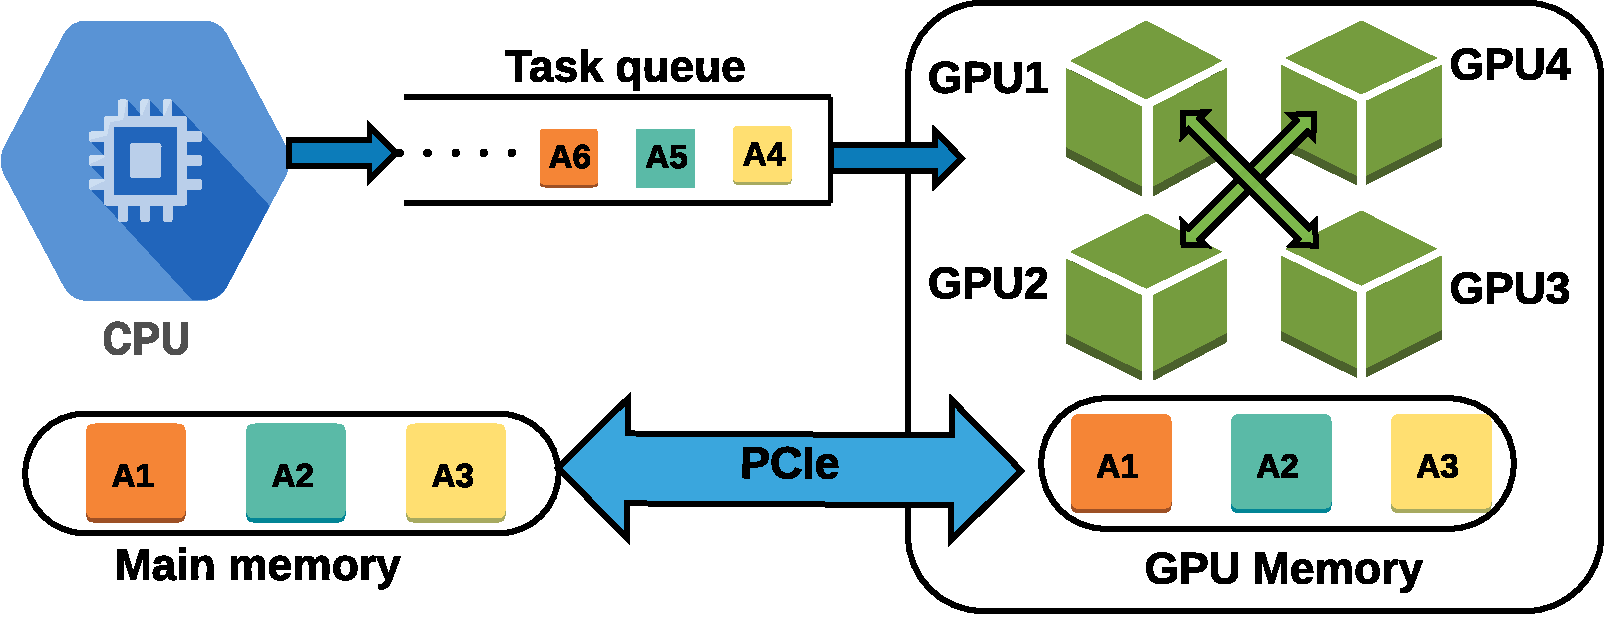
\includegraphics[width=.84\linewidth,height=2.2cm]{figs/cpu-gpu-queue.pdf}
  \vspace{-2mm}
  \caption{Application queue on a single node with multiple GPUs.}
  \vspace{-2mm}
  \label{fig:queue}
\end{figure}

% For example, a wearable health monitoring device aggregates several sensor data through a mobile application. In case of a data anomaly, inference services can be triggered from the mobile device to the cloud, requesting for a deep neural network  (DNN) model that fits the symptom \cite{hauswald2015djinn}. 

A class of emerging workloads in public datacenters, which include user-facing queries (in forms of voice, text and image etc.)  \cite{qualcomm,TjongKimSang:2000:ICS:1117601.1117631,Hearst:2011:NSU:2018396.2018414}, demand sub-millisecond turn around times (such as Siri and Alexa) \cite{siri,alexa} and pose varying compute demands \cite{Hauswald:2015:SOE:2694344.2694347}. These applications, subscribe to datacenter accelerators in the form of queries (e.g. inference requests from a DNN model) \cite{hauswald2015djinn}. These GPU-bound queries impose strict Service Level Agreements (SLAs) that is usually set around 150 to 500ms~\cite{gujarati2017swayam}. In contrast to the regular datacenter batch workloads, these user-facing applications are typically hosted as services that occur and scale in short bursts \cite{Barroso:2009:DCI:1643608,Dean}. Companies like Netflix break down their application compute flow pipeline into several containerized microservices in order to ease scalability and maintenance of the workflow  ~\cite{netflix}. Many of these containerized workloads and microservices subscribe to compute-intensive frameworks such as Tensorflow~\cite{tensor}, Caffe~\cite{jia2014caffe}, Theano~\cite{Theano}, etc. taking advantage of GPU's high performance API primitives~\cite{ChetlurWVCTCS14}. Note that, these microservices are interconnected with each stage having strict deadlines depends on the application scheduler to meet the tight performance bounds. With the expected increase in such workloads~\cite{cisco}, the GPU resource scheduling problem is expected to exacerbate. Hence, GPUs/accelerators are on the critical path to ensure the performance, and meet end-to-end latency demands of such queries.
% MATLAB \cite{Dean,Weideman:2000:MDM:365723.365727},

Also, we identify that the GPU-agnostic orchestration and scheduling would violate the strict QoS deadline of these queries. As a result, an efficient management strategy of such compute accelerators across the datacenter becomes crucial. 
%For example, Google Brain project \cite{brain}, which is a DNN based containerized service, is used across teams in Google to reduce the need to maintain different implementations of the same service. This trend is also increasingly common in companies like 
On the other hand, these services if not batched together would also underutilize the GPU~\cite{hauswald2015djinn}. The primary design goal of any efficient cluster manager is to achieve high resource utilization with low job turnaround times. Traditional datacenter operators leverage techniques such as hardware virtualization \cite{Gupta:2011:PCS:2002181.2002184} to improve the overall cluster utilization. To further improve the energy efficiency, the cluster resource orchestrators also employ techniques like workload consolidation or dynamic load balancing through VM migration. However, none of these traditional CPU-based cluster management techniques can be extended to GPU-based datacenters since commodity GPUs can neither be virtualized nor be consolidated because the jobs scheduled to GPUs are not preemptible.\footnote{GPU virtualization in Nvidia Grid is only for graphics pipeline \cite{grid}.}

State-of-the-art resource orchestrators such as Kubernetes \cite{kubernetes} and Mesos \cite{mesos} perform uniform scheduling, which statically assigns the GPU resources to the applications. The scheduled pods access the GPUs via PCIe pass-through, which gives the application complete access to the GPU as seen in Figure~\ref{fig:queue}. Specifically, Kubernetes has support for dynamic orchestration with features such as node affinity, pod\footnote{We use the terms (Google's) pod and container interchangeably.} affinity, and pod preemption for CPUs. However, these features cannot be extended to GPUs as they lack support for pod preemption. In addition, \textit{Kubernetes} lacks the ability to query real-time GPU metrics such as memory, Streaming Multiprocessor(SM is a GPU-core) utilization, PCIe bandwidth, etc. Containers often overstate their GPU resource requirements such as memory, and this leads to severe resource underutilization and QoS violations due to queuing delays~\cite{kang2017convgpu}. To summarize, we list several challenges in managing GPU based datacenters below, %Hence we need to build an orchestration layer which can log the critical metrics and use them with state of the art Kubernetes features to develop a utilization aware and. \jash{strongly mention util problem and emphasize your takeaways} %Since the resource management layer has no control over the GPU utilization or management, the resource fairness is entirely dependent on the application which is currently running on GPU. Hence techniques such as preemption to enforce fairness cannot be applicable in this case.%



% The default scheduling options in kubernetes or Mesos are tuned towards optimizing CPU cluster metrics such as throughput, and overall resource utilization. These schedulers are also agnostic to the heterogeneity available in these architectures, and therefore, lead to suboptimal scheduling.
% However these resource orchestrators like Kubernetes also have provision to plug-in custom scheduling policies based on the specific demands of the datacenter. We propose a need for GPU focused datacenter cluster orchestrator. To meet this need, we discuss the potential challenges in designing a GPU context aware scheduler by exposing the device API's to the kubernetes.


\begin{itemize}[wide, nosep, labelindent = 0pt, topsep = 0.3ex]
\item \textbf{Non-preemptive processing elements -} The containers scheduled to GPUs cannot be preempted, or context switched, or prioritized and are scheduled based on First Come First Serve (FCFS) order~\cite{amert2017gpu} as seen in Figure~\ref{fig:queue}. Therefore, GPU-bound latency sensitive queries when queued behind a batch job will incur severe queuing delays.

\item \textbf{GPU utilization aware scheduler -} Today's datacenter resource orchestrators treat GPU's as a black box and are agnostic of GPU utilization metrics. Meeting the QoS of a latency sensitive query is difficult without knowing the system state, especially when it is shared.

\item \textbf{Unaccountable container performance metrics -} \\Container-level accountability for resource consumption is not enabled in GPUs. This lets the node-level application frameworks like Tensorflow to conservatively over-commit the GPU resources~\cite{tensorflowgpu} resulting in poor energy efficiency %due to resource underutilization.
\item \textbf{Performance per watt proportionality -} GPUs have linear performance per watt scaling, which implies that the maximum energy efficiency can be achieved only when GPUs are 100\% utilized, unlike CPUs \cite{wong2016peak}. It is crucial for a scheduler to fully pack and utilize the GPUs without affecting the individual application performance.
\end{itemize}

\begin{figure}[!tbp]
\centering
  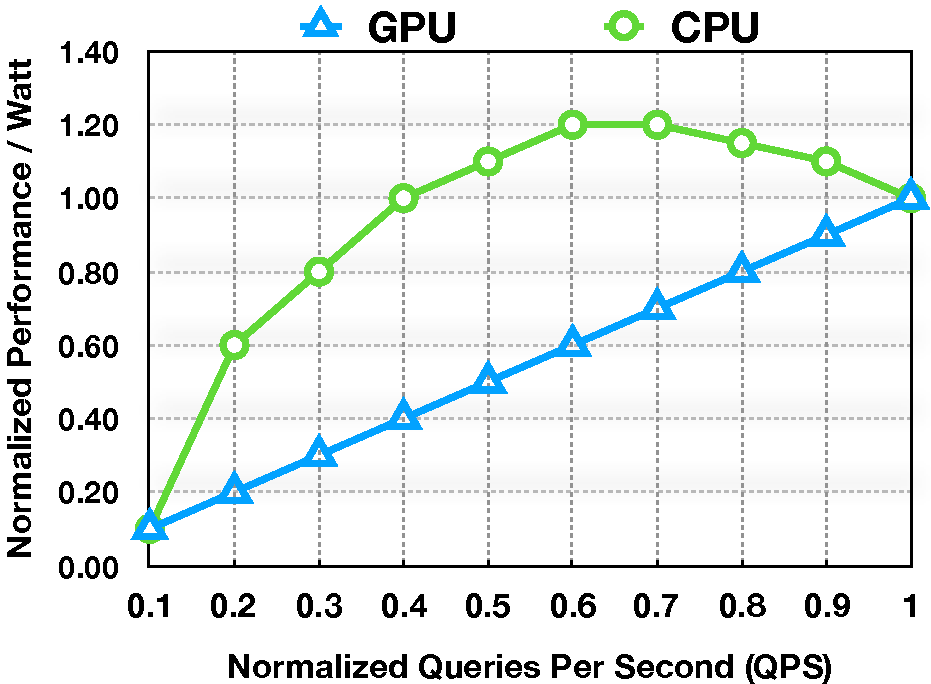
\includegraphics[width=.85\linewidth]{results/energy.pdf}
  \vspace{-2mm}
  \caption{Performance per Watt trend of CPU and GPU serving Memcached queries.}
  \vspace{-2mm}
  \label{fig:efficiency}
\end{figure}

% The challenges listed above pitches a strong case for reducing resource fragmentation through workload consolidation. In case of co-located GPU applications, prediction of the end-to-end latency and QoS of a query becomes difficult. %The schedulers today are agnostic of accelerator device metrics and without specific orchestration or scheduling policy in place, schedulers treat the accelerators as black boxes. They schedule the queries based on FCFS without any bounded performance guarantees. Such resource-agnostic, conservative scheduling policies lead to poor utilizations and are also energy inefficient. 
% \begin{figure*}
% \hspace{-10mm}
% \begin{subfigure}[t!]{.3\textwidth}
%   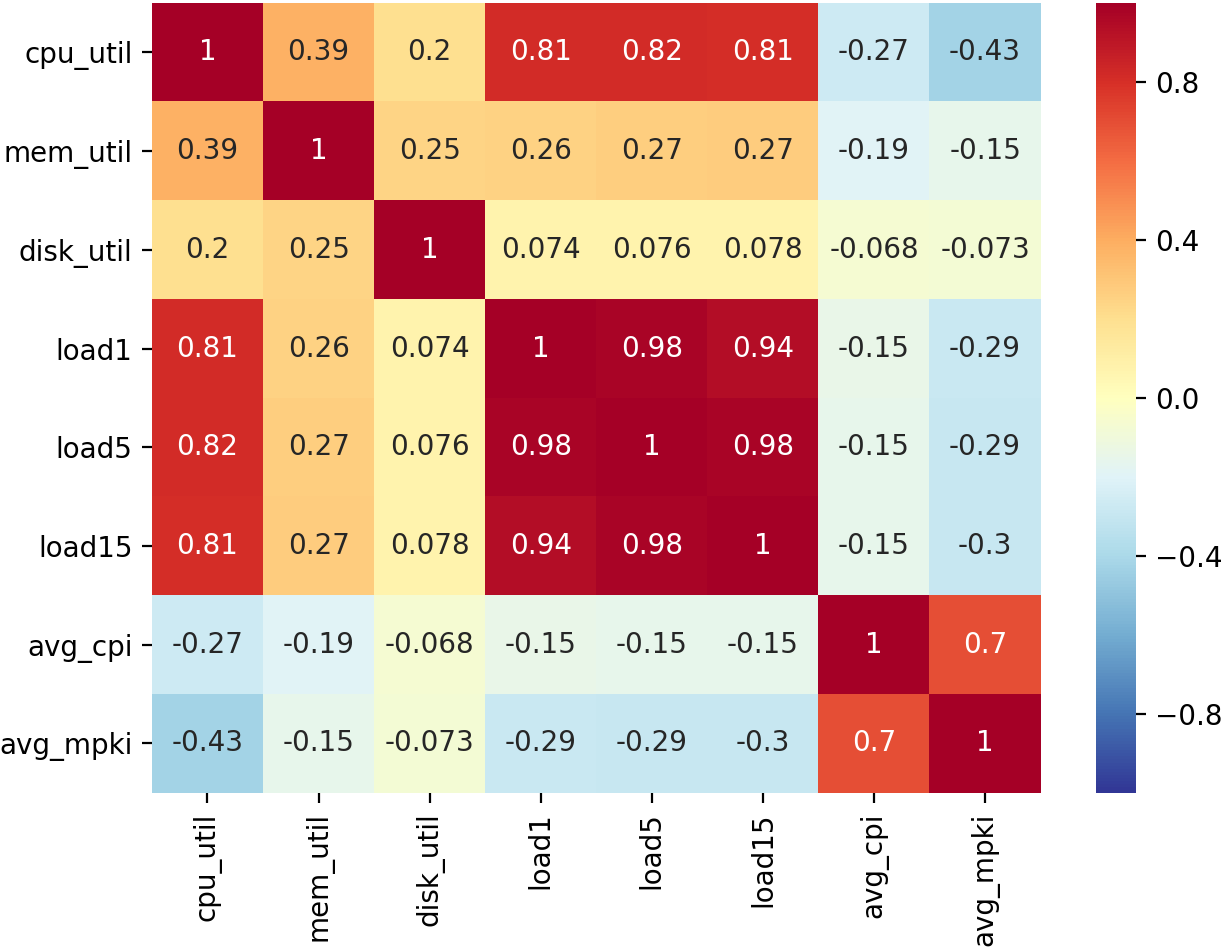
\includegraphics[width=.9\linewidth]{results/container_usage.png}
%   \caption{Latency-critical task's usage metrics}
%   \label{fig:container}
%  \end{subfigure}%
 
%   \begin{subfigure}[t!]{0.32\textwidth}
%   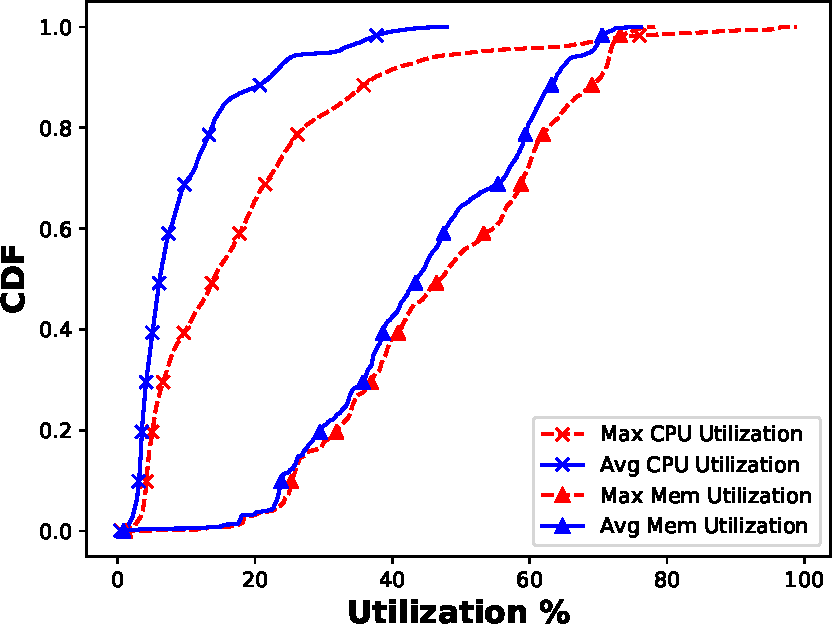
\includegraphics[width=.9\linewidth]{results/cdf.pdf}
%   \caption{Average \& Maximum CPU and memory utilization of latency-critical containerized production services.}
%   \label{fig:cont-mem}
% \end{subfigure}%

%   \begin{subfigure}[t!]{0.3\textwidth}
%   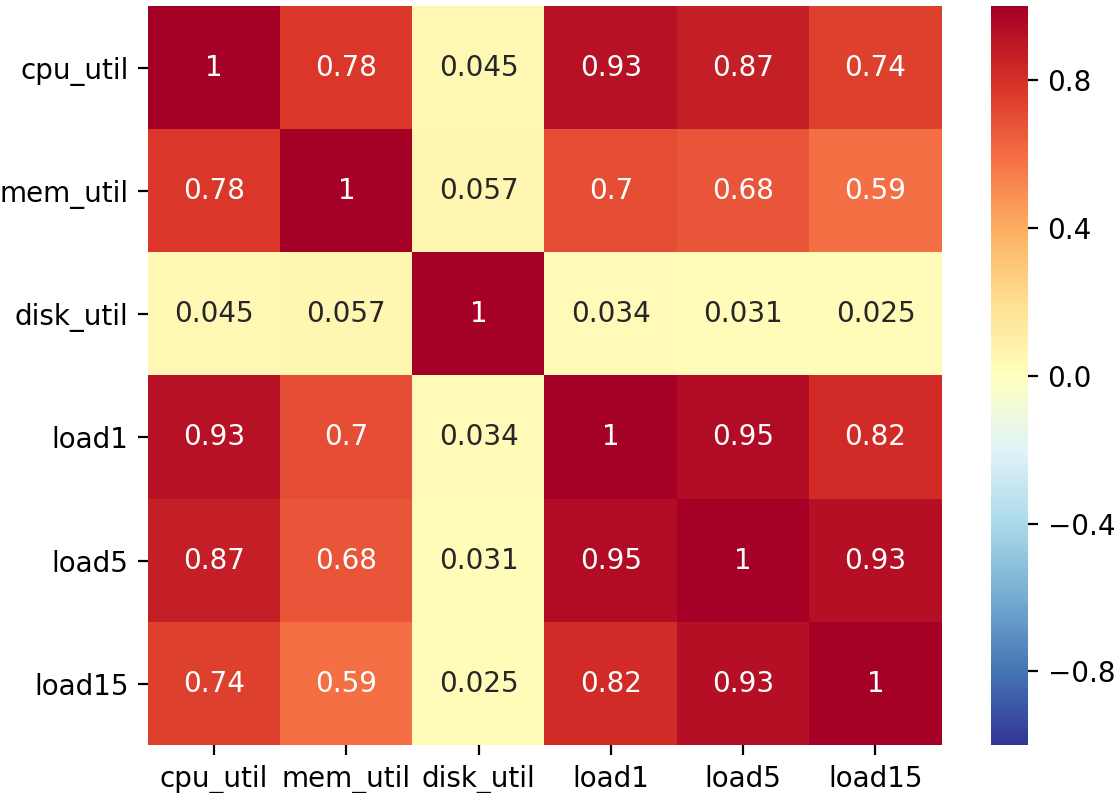
\includegraphics[width=.9\linewidth]{results/batch_usage.png}
%   \hspace{2mm}
%   \caption{Long running batch task's usage metrics}
%   \label{fig:batch}
% \end{subfigure}%
% \vspace{-2mm}
% \caption{Alibaba trace analysis of resource utilization of 1300 machines across 12,951 batch jobs \& 11,089 containers (12hr period).}
% \label{fig:ali}
% \end{figure*}

\begin{figure*}
\hspace{-10mm}
\begin{subfigure}[t!]{.42\textwidth}
  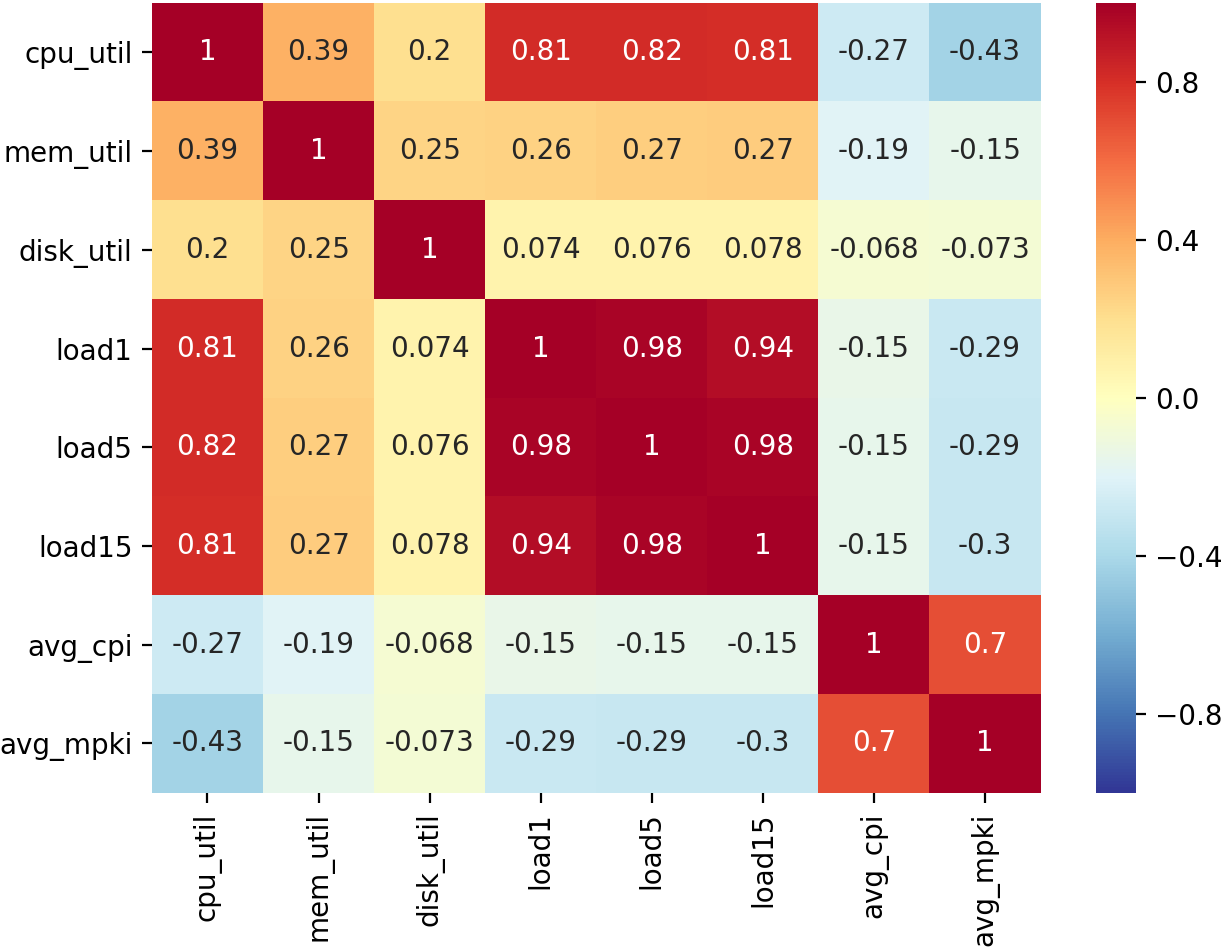
\includegraphics[width=.99\linewidth ,height=5.3cm, width=6.7cm]{results/container_usage.png}
  \caption{Latency-critical task's usage metrics}
  \label{fig:container}
 \end{subfigure}%
 \hspace{-5mm}
  \begin{subfigure}[t!]{0.3\textwidth}
  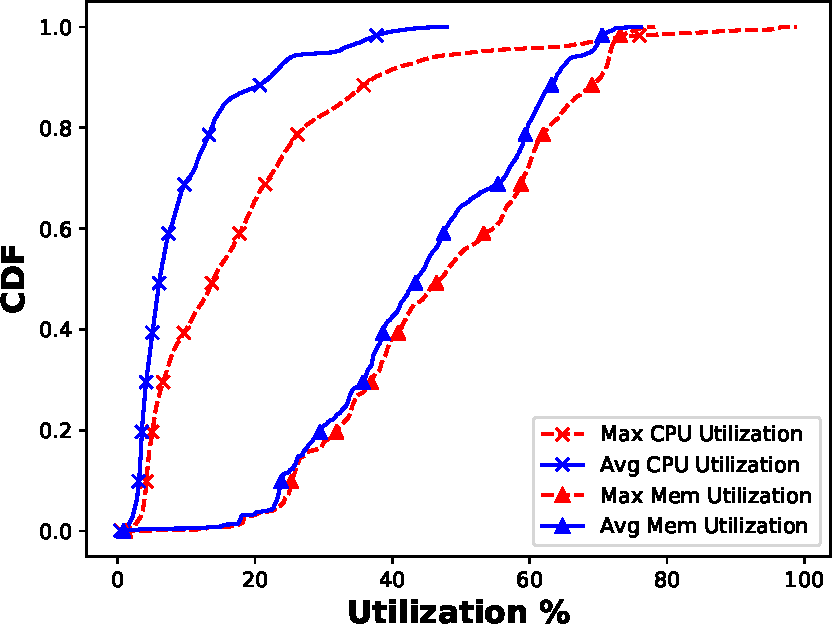
\includegraphics[width=.99\linewidth,height=4.5cm, width=5.3cm]{results/cdf.pdf}
  \caption{Average \& Maximum CPU and memory utilization of latency-critical containerized production services.}
  \label{fig:cont-mem}
\end{subfigure}%
  \begin{subfigure}[t!]{0.33\textwidth}

  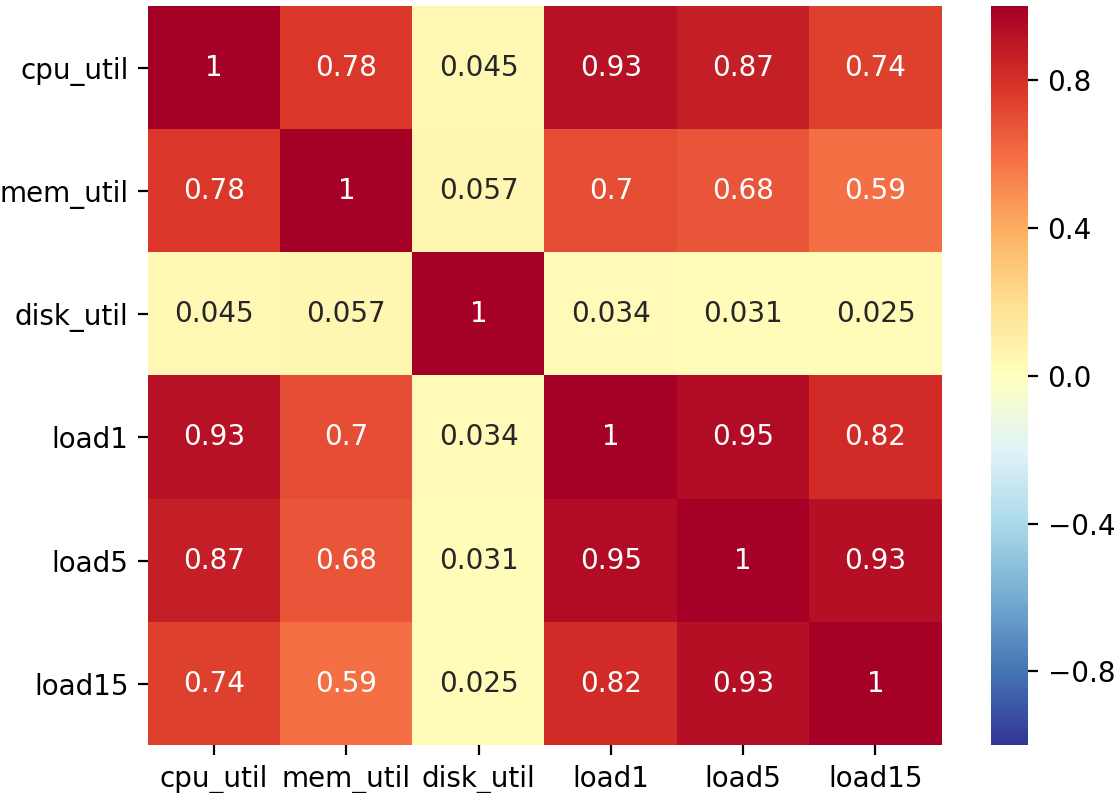
\includegraphics[width=.99\linewidth, height=4.8cm,width=6.4cm]{results/batch_usage.png}
  \hspace{2mm}
  \caption{Long running batch task's usage metrics}
  \label{fig:batch}
\end{subfigure}%
\vspace{-2mm}
\caption{Alibaba trace analysis of resource utilization of 1300 machines across 12,951 batch jobs \& 11,089 containers (12hr period).}
\label{fig:ali}
\end{figure*}

As a result, there is an inherent need for a GPU utilization-aware resource orchestration along with qos-aware job scheduler. In this paper, we propose \textit{Kube-Knots}\footnote{Google's \textit{Kubernetes} means helmsman or captain of the ship managing multiple containers. In \textit{Kubernetes},  \textit{Knots} orchestrates the scheduling speed of the accelerated containers.} by integrating \textit{Knots}, a GPU aware orchestration layer with \textit{Kubernetes}. Integrating \textit{Knots} with \textit{Kubernetes} enables GPU-aware resource orchestration used alongside with existing job schedulers to schedule for both CPU and GPU specific workloads. Since there is significant work done towards utilization aware CPU scheduling  \cite{Tang:2013:RRS:2451116.2451126,Marsbubbleup,Yang:bubbleflux}, in this paper, we focus only on scheduling for GPU specific workloads. Using \textit{Kube-Knots}, we make the following contributions:
\\
\begin{enumerate}[wide = 0pt, labelwidth = 1.3em, labelsep*=0em, itemindent = 0pt, leftmargin = \dimexpr\labelwidth + \labelsep\relax, noitemsep,topsep = 1ex, font=\normalfont]

\item \textit{Knots}, is a GPU resource orchestrator which works with a node-level GPU resource manager to monitor the real-time GPU utilization metrics at every node.

\item We generate datacenter representative GPU cluster workloads to evaluate our proposed schedulers on a ten node GPU cluster managed by \textit{Kubernetes} with \textit{Knots}.

\item We build three schedulers namely Resource Agnostic (Res-Ag), Correlation Based Prediction (CBP), and Peak Prediction (PP) that leverage the cluster-wide GPU utilization time-series data aggregated from \textit{Kube-Knots}.

%\item Cluster-wide GPU metrics are collected by the utilization aggregator at headnode, and the time-series data is used for future GPU scheduling decisions. Thus enabling \textit{Kube-Knots} to make GPU-utilization aware resource orchestration.

\item Our proposed CBP scheduler uses GPU usage correlation metrics to perform safe pod co-locations ensuring crash-free container resizing and efficient packing on GPUs.

\item CBP along with PP scheduler can guarantee the end-to-end QoS of latency critical queries by predicting loads of GPUs through ARIMA~\cite{arima} based time-series forecasting. This further reduces the QoS violations by up to 53\% when compared to the resource agnostic scheduler.

\item \textit{Kube-Knots}\footnote{We plan to release \textit{Kube-Knots} as an open-source plug-in patch for \textit{Kubernetes}, that could be leveraged by the community to dynamically orchestrate GPU-based containers via Kubernetes.} improves the cluster-wide GPU utilization through performance-aware workload consolidation by up to 80\%  for both 50$^{th}$ and 90$^{th}$ percentile utilization when compared to resource agnostic scheduler. Thus reducing the datacenter wide GPU energy consumption by 33\% on an average when compared against GPU agnostic orchestration.

\end{enumerate}

